% Options for packages loaded elsewhere
\PassOptionsToPackage{unicode}{hyperref}
\PassOptionsToPackage{hyphens}{url}
%
\documentclass[
  11pt,
]{article}
\usepackage{amsmath,amssymb}
\usepackage{lmodern}
\usepackage{iftex}
\ifPDFTeX
  \usepackage[T1]{fontenc}
  \usepackage[utf8]{inputenc}
  \usepackage{textcomp} % provide euro and other symbols
\else % if luatex or xetex
  \usepackage{unicode-math}
  \defaultfontfeatures{Scale=MatchLowercase}
  \defaultfontfeatures[\rmfamily]{Ligatures=TeX,Scale=1}
\fi
% Use upquote if available, for straight quotes in verbatim environments
\IfFileExists{upquote.sty}{\usepackage{upquote}}{}
\IfFileExists{microtype.sty}{% use microtype if available
  \usepackage[]{microtype}
  \UseMicrotypeSet[protrusion]{basicmath} % disable protrusion for tt fonts
}{}
\makeatletter
\@ifundefined{KOMAClassName}{% if non-KOMA class
  \IfFileExists{parskip.sty}{%
    \usepackage{parskip}
  }{% else
    \setlength{\parindent}{0pt}
    \setlength{\parskip}{6pt plus 2pt minus 1pt}}
}{% if KOMA class
  \KOMAoptions{parskip=half}}
\makeatother
\usepackage{xcolor}
\usepackage[margin=1in]{geometry}
\usepackage{graphicx}
\makeatletter
\def\maxwidth{\ifdim\Gin@nat@width>\linewidth\linewidth\else\Gin@nat@width\fi}
\def\maxheight{\ifdim\Gin@nat@height>\textheight\textheight\else\Gin@nat@height\fi}
\makeatother
% Scale images if necessary, so that they will not overflow the page
% margins by default, and it is still possible to overwrite the defaults
% using explicit options in \includegraphics[width, height, ...]{}
\setkeys{Gin}{width=\maxwidth,height=\maxheight,keepaspectratio}
% Set default figure placement to htbp
\makeatletter
\def\fps@figure{htbp}
\makeatother
\setlength{\emergencystretch}{3em} % prevent overfull lines
\providecommand{\tightlist}{%
  \setlength{\itemsep}{0pt}\setlength{\parskip}{0pt}}
\setcounter{secnumdepth}{-\maxdimen} % remove section numbering
\newlength{\cslhangindent}
\setlength{\cslhangindent}{1.5em}
\newlength{\csllabelwidth}
\setlength{\csllabelwidth}{3em}
\newlength{\cslentryspacingunit} % times entry-spacing
\setlength{\cslentryspacingunit}{\parskip}
\newenvironment{CSLReferences}[2] % #1 hanging-ident, #2 entry spacing
 {% don't indent paragraphs
  \setlength{\parindent}{0pt}
  % turn on hanging indent if param 1 is 1
  \ifodd #1
  \let\oldpar\par
  \def\par{\hangindent=\cslhangindent\oldpar}
  \fi
  % set entry spacing
  \setlength{\parskip}{#2\cslentryspacingunit}
 }%
 {}
\usepackage{calc}
\newcommand{\CSLBlock}[1]{#1\hfill\break}
\newcommand{\CSLLeftMargin}[1]{\parbox[t]{\csllabelwidth}{#1}}
\newcommand{\CSLRightInline}[1]{\parbox[t]{\linewidth - \csllabelwidth}{#1}\break}
\newcommand{\CSLIndent}[1]{\hspace{\cslhangindent}#1}
\usepackage{setspace}\doublespacing
\usepackage{lineno}\linenumbers
\usepackage[utf8]{inputenc}
\usepackage[T1]{fontenc}
\usepackage{biblatex}
\usepackage{booktabs}
\usepackage{longtable}
\usepackage{array}
\usepackage{multirow}
\usepackage{wrapfig}
\usepackage{float}
\usepackage{colortbl}
\usepackage{pdflscape}
\usepackage{tabu}
\usepackage{threeparttable}
\usepackage{threeparttablex}
\usepackage[normalem]{ulem}
\usepackage{makecell}
\usepackage{xcolor}
\ifLuaTeX
  \usepackage{selnolig}  % disable illegal ligatures
\fi
\IfFileExists{bookmark.sty}{\usepackage{bookmark}}{\usepackage{hyperref}}
\IfFileExists{xurl.sty}{\usepackage{xurl}}{} % add URL line breaks if available
\urlstyle{same} % disable monospaced font for URLs
\hypersetup{
  pdftitle={Evolution along allometric lines of least resistance: Morphological differentiation in Pristurus geckos},
  hidelinks,
  pdfcreator={LaTeX via pandoc}}

\title{Evolution along allometric lines of least resistance:
Morphological differentiation in \emph{Pristurus} geckos}
\author{}
\date{\vspace{-2.5em}}

\begin{document}
\maketitle

\begin{center}
\textbf{H{\'{e}}ctor Tejero-Cicu{\'{e}}ndez$^{1,*}$,  Iris Men{\'{e}}ndez$^{2}$, Adri{\'{a}}n Talavera$^{1}$, Gabriel Riaño$^{1}$, Bernat Burriel-Carranza$^{1}$, Marc Sim{\'{o}}-Riudalbas$^{1}$, Salvador Carranza$^{1}$, and Dean C. Adams$^{3}$}
\end{center}

\begin{center}22 November, 2022\end{center}

\(^{1}\)Institute of Evolutionary Biology (CSIC-Universitat Pompeu
Fabra), Passeig Marítim de la Barceloneta 37-49, Barcelona 08003, Spain

\(^{2}\)Museum für Naturkunde, Leibniz Institute for Evolution and
Biodiversity Science, Berlin, Germany

\(^{3}\)Department of Ecology, Evolution, and Organismal Biology, Iowa
State University, Ames, Iowa, 50010 USA

\(^{*}\)Correspondence: Héctor Tejero-Cicuéndez
\href{mailto:cicuendez93@gmail.com}{\nolinkurl{cicuendez93@gmail.com}}

\newpage

\hypertarget{abstract}{%
\section{Abstract}\label{abstract}}

Species living in distinct habitats often experience unique ecological
selective pressures, which can drive phenotypic divergence. However, how
ecophenotypic patterns are affected by allometric trends and trait
integration levels is less well understood. Here we evaluate the role of
allometry in shaping patterns of body size and shape diversity in
\emph{Pristurus} geckos utilizing differing habitats. We found that
patterns of body shape allometry and integration were distinct in
species utilizing differing habitats, with ground-dwelling
\emph{Pristurus} displaying the most divergent allometric trend and the
strongest integration. There was also strong concordance between static
allometry across individuals and evolutionary allometry among species,
revealing that body shape differences among individuals were predictive
of evolutionary changes across the phylogeny at macroevolutionary
scales. This suggested that phenotypic evolution occurred along
allometric lines of least resistance, with allometric trajectories
imposing a strong influence on the magnitude and direction of size and
shape changes across the phylogeny. When viewed in phylomorphospace, the
largest rock-dwelling species were most similar in body shape to the
smallest ground-dwelling species, and vice versa. Thus, in
\emph{Pristurus}, phenotypic evolution along the differing habitat-based
allometric trajectories resulted in similar body shapes at differing
body sizes in distinct ecological habitats.

\newpage

\hypertarget{introduction}{%
\section{1. Introduction}\label{introduction}}

Understanding how phenotypic diversity evolves, and elucidating the
forces that generate and maintain this diversity, are major goals in
evolutionary biology. Because adaptive evolution is the product of
natural selection, changes in ecological selection pressures are
expected to affect the evolutionary trajectory of phenotypic traits that
facilitate an organism's survival in their habitat. Evolutionary theory
predicts that differing habitats will exert unique ecological selection
pressures on organisms, resulting in associations between ecological and
phenotypic traits. Indeed, species inhabiting differing habitats often
display functional, behavioral, or phenotypic differences, that have
presumably been the result of adaptive diversification in their
respective ecological contexts {[}1--5{]}. \hfill\break

One possible evolutionary outcome of ecological specialization is that
organisms inhabiting similar environments display common phenotypic
characteristics. When such patterns occur repeatedly {[}6,7{]}, this
convergent evolution is treated as strong evidence of adaptation. Indeed
the ecomorphological paradigm {[}8{]} is predicated, in part, on such
cases, which emphasize the strong association between the phenotypic
traits that organisms display (morphological, behavioral, or
physiological) and the ecological characteristics of their habitat that
mediate organismal performance. In vertebrates, ecomorphological trends
have been well studied in numerous taxonomic groups, and include the
emblematic `ecomorphs' of Caribbean \emph{Anolis} lizards that exploit
different microhabitats {[}6,9,10{]}, differential beak morphology in
species of Darwin's finches {[}11--13{]}, the recurring phenotypes of
African lake cichlids across ecological regimes {[}14,15{]}, and the
distinct body forms of freshwater fishes in benthic and limnetic
habitats {[}16--18{]}, among others. \hfill\break

However, while the patterns of morphological differences in distinct
ecological contexts have been well documented, less-well understood is
how this differentiation has been influenced by trait covariation
associated with body size differences (i.e., allometry). Evaluating
allometric trends across hierarchical levels (e.g., comparing allometry
at the individual level, or static allometry, and among species, or
evolutionary allometry) may aid in our understanding of how adaptive
morphological change occurs at macroevolutionary scales {[}19{]}. It has
long been recognized that the interrelationships among traits can exert
a strong influence on how phenotypic evolution proceeds, as trait
correlations influence the degree to which phenotypic variation is
exposed to selection {[}20{]}. Thus, the integration among traits can
constrain phenotypic change in certain directions, or enhance variation
along other phenotypic axes {[}20--27{]}. Further, because nearly all
linear traits covary strongly with overall body size {[}28,29{]},
allometric trends could be considered the quintessential expression of
phenotypic integration. Thus, identifying whether allometric patterns
differ across habitats, and how such patterns of trait covariation
affect ecomorphological trends among species utilizing those habitats,
remains an important question worthy of investigation. \hfill\break

The Afro-Arabian geckos in the genus \emph{Pristurus} afford the
opportunity to elucidate the interdigitating effects of allometry and
habitat specialization on clade-level patterns of phenotypic diversity.
Prior work on this system {[}30{]} revealed that the colonization of
ground habitats has been a trigger of morphological change, specifically
reflected in an increase in body size and shape disparity.
Interestingly, some ground-dwelling species are among the largest of the
genus and also show increased relative head sizes and limb proportions,
while some other species with this ecological specialization have
evolved to be among the smallest of the group. Additionally, among the
species exploiting rocky habitats (the most common ecological feature in
\emph{Pristurus}), there are also species with both considerably large
and small body sizes {[}30{]}. What remains unexplored, however, is how
the evolution of body shape is related to differences in body size and
whether habitat specialization has an impact in this shape-size
relationship. \hfill\break

In this study, we employed a combination of multivariate morphometric
and phylogenetic comparative analyses to interrogate macroevolutionary
patterns of evolutionary allometry in \emph{Pristurus} geckos of
Afro-Arabia. Using phenotypic, phylogenetic, and ecological data, we
first characterized allometric trends in body form in the group, to
discern the extent to which evolutionary allometric trends across the
phylogeny aligned with habitat-based static allometry for species
occupying distinct ecological regimes. We then examined changes in
allometric trends across the phylogeny, and linked these patterns to
overall phenotypic integration, diversification in morphospace, and
habitat utilization among taxa. Our analyses reveal that patterns of
evolutionary allometry across species align with allometric trends
within habitats, demonstrating that the interplay between ecological
specialization and allometric trajectories in species with disparate
body size may play a determinant role in shaping the phenotypic
evolution and hence in adaptive dynamics in this clade.

\hypertarget{materials-and-methods}{%
\section{2. Materials and Methods}\label{materials-and-methods}}

\hypertarget{a-data}{%
\subsection{(a) Data}\label{a-data}}

We used a combination of phenotypic, phylogenetic, and ecological data
to characterize and evaluate intra- and interspecific allometric trends.
The data utilized here were obtained from our prior work on this system
{[}30,31{]}, and are briefly described here. First we used a time-dated,
molecular phylogeny of squamates that included all members of the genus
\emph{Pristurus}, including several currently undescribed taxa. The tree
was estimated in a Bayesian framework, using five mitochondrial markers,
six nuclear markers, and 21 calibration points {[}31{]}. Next we
categorized each species as belonging to one of three ecological groups
(ground, rock, or tree), based on descriptions of habitat use found in
the literature {[}30{]}. Finally, we obtained a phenotypic data set
containing body size (snout-vent length: SVL) and eight linear
measurements (Figure 1) that described overall body form: trunk length
(TrL), head length (HL), head width (HW), head height (HH), humerus
length (Lhu), ulna length (Lun), femur length (Lfe), and tibia length
(Ltb) {[}30{]}. We restricted our study to those species represented by
nine or more individuals; resulting in a dataset of 687 individuals from
25 species (invidivuals per species: \(\mu=27\); min = 9, max = 56).
Species in the phenotypic dataset were then matched to the phylogeny,
which was subsequently pruned to arrive at the final topology. All
measurements were log-transformed prior to statistical analyses.
Additional details regarding data collection and formal descriptions of
each linear measurement may be found in the original sources
{[}30,31{]}. The data are available on DRYAD:
\url{https://doi.org/10.5061/dryad.xwdbrv1f6} {[}32{]}.

\hypertarget{b-statistical-and-comparative-analyses}{%
\subsection{(b) Statistical and Comparative
Analyses}\label{b-statistical-and-comparative-analyses}}

We conducted a series of analyses to interrogate allometric trends,
patterns of integration, and macroevolutionary changes in allometry,
relative to differentiation in body form. First we characterized
evolutionary allometry in the genus by performing a phylogenetic
multivariate regression of body form on body size (i.e., SVL), using the
species means as data. We then performed an analogous procedure at the
individual level, regressing body form on body size using our entire
dataset. From both the species-level (phylogenetic) and the
individual-level analyses, we obtained the set of regression
coefficients, and calculated the difference in their angular direction
to describe the extent to which patterns of allometry at the individual
level were concordant with evolutionary allometric trends across
species. \hfill\break

Next we used the dataset containing all individuals to determine whether
trends in static allometry differed across habitat groups. This was
accomplished by performing a multivariate analysis of covariance, with
body size (\(SVL\)), \(habitat\), and \(SVL\times habitat\) as model
effects. Significance was evaluated using 999 iterations of a
permutation procedure, where residuals from a reduced model were
randomly permuted in each permutation (RRPP), model statistics were
recalculated, and used to generate empirical null sampling distributions
to evaluate the observed test statistics {[}following 33,34,35{]}. We
then compared the multivariate allometric vectors for each habitat group
to one another, and to a vector representing multivariate isometry, by
calculating pairwise differences in their angular direction in
morphospace, and evaluating these relative to empirical sampling
distributions obtained through RRPP {[}34,36,37{]}. Here, residuals were
obtained from a common isometry reduced model, whose common slope
component described a pattern of multivariate isometry, and whose
intercepts allowed for differences in least-squares means among groups.
Patterns of multivariate allometry relative to body size were visualized
via regression scores {[}38{]} and predicted lines {[}39{]}, based on
the coefficients and fitted values from the linear model described
above. \hfill\break

Additionally, because allometry describes the extent to which traits
covary with body size and with each other (i.e., integration), we
conducted an analysis of integration. Here we characterized the extent
of morphological integration in body form for individuals within each
habitat group by summarizing the dispersion of eigenvalues of their
respective trait covariance matrix {[}40{]}. This measure (\(V_{rel}\))
was subsequently converted to an effect size (a \(Z\)-score), which
quantified the strength of morphological integration {[}41{]}. We then
performed a series of two-sample tests to compare the strength of
morphological integration across habitat groups, following the
procedures of {[}41{]}. Additionally and for comparison, we repeated
these analyses on the set of size-standardized trait data, found as a
set of shape ratios {[}42{]} where each trait was divided by body size
(Supplementary Material). \hfill\break

To determine the extent to which static and evolutionary allometry were
concordant, we evaluated the directions in morphospace of both the
evolutionary (species-level) and static (habitat-based) allometric
trends. Specifically, we obtained the set of regression coefficients
from both the phylogenetic multivariate regression and the multivariate
analysis of covariance analyses above, and calculated the differences in
angular direction between the evolutionary trajectory and the static
allometry trend for each habitat group. The observed angles were then
statistically evaluated relative to empirical sampling distributions
obtained through permutation (RRPP), based on the common isometry model
described above. \hfill\break

Next, to discern how allometric trends resulted in the evolution of
distinct body forms, we examined changes in the body shape proportions
across the phylogeny. Here we treated the head dimensions and limb
dimensions separately, as allometric trends could potentially differ
between these body regions due to differential functional or selective
constraints {[}43{]}. Because both the head and limb data were
multivariate, we first performed a partial least squares (PLS) analysis
{[}44{]} of the head traits versus SVL, and the limb traits versus SVL,
to describe the direction of maximal covariation between each body
region and size. We then measured the mean residuals of each species to
the inferred allometric trend, which described the extent to which head
and limb proportions of species were greater or smaller than expected
for their body size. The species residuals were then mapped on the
phylogeny of \emph{Pristurus} using a Brownian motion model of
evolution, to qualitatively evaluate shifts in head and limbs
proportionality across the phylogeny for the group. Similarly,
within-species patterns of static allometry were visualized by plotting
regressions of PLS scores on SVL for both head and limb traits
separately. \hfill\break

Finally, to relate within-species allometric trends with patterns of
phenotypic diversification in the group we generated a phylomorphospace,
based on a phylogenetic principal component analyses (PCA) on the
size-standardized species means obtained from a phylogenetic regression
{[}see 30{]}. Here, phenotypic similarities among species, relative to
their phylogenetic relationships and habitat affiliations, were
observed. Additionally, representative specimens (scaled to unit size)
were also visually compared to aid in describing these trends. A similar
phylomorphospace was constructed for species means not corrected for
body size, and the phenotypic disparity among species means in each
habitat was calculated and subsequently compared (Supplementary
Material). All analyses were conducted in R 4.2.1 {[}45{]}, using
\texttt{RRPP} version 1.3.1 {[}46,47{]} and \texttt{geomorph} 4.0.4
{[}48{]} for statistical analyses and the \texttt{tidyverse} version
1.3.0 {[}49{]}, \texttt{phytools} version 0.7-77 {[}50{]}, and a
modified version of the function \texttt{ggphylomorpho}
{[}\url{https://github.com/wabarr/ggphylomorpho}{]} for data
manipulation and visualization, as well as scripts written by the
authors (Supplementary Material).

\hypertarget{results}{%
\section{3. Results}\label{results}}

Using phylogenetic regression, we found significant evolutionary
allometry in body form across species (\(N_{sp}=25\); \(F = 217.9\);
\(Z =5.53\); \(P < 0.001\)). Likewise, when allometry in body form was
examined across individuals, a similar pattern was observed
(\(N_{ind}=687\); \(F = 7910.8\); \(Z =9.20\); \(P < 0.001\)). Further,
the vectors of regression coefficients between the two analyses were
highly correlated (\(\rho = 0.94\)) and were oriented in nearly parallel
directions in morphospace (\(\theta = 1.49^\circ\)). This revealed that
the pattern of multivariate allometry across individuals was concordant
with macroevolutionary trends of interspecific allometry among species
of \emph{Pristurus} across the phylogeny. \hfill\break

Our analyses also exposed significant differences in the allometry of
body form among \emph{Pristurus} utilizing distinct habitats (Table 1).
Further, pairwise comparisons of multivariate allometric vectors
revealed that patterns of static allometry in each habitat differed
significantly from isometry, indicating the presence of multivariate
allometry in each (Table 2). Additionally, comparisons identified that
ground-dwelling \emph{Pristurus} displayed the most distinct allometric
trend as compared with \emph{Pristurus} occupying both the rock and tree
habitats (Table 2; Figure 2). Here, regression coefficients of each
trait versus size (Supplementary Material) revealed that ground-dwelling
\emph{Pristurus} exhibited strong positive allometry for all head and
limb traits (i.e., \(\beta>1.0\)). By contrast, rock and tree-dwelling
\emph{Pristurus} displayed negative allometry (i.e., \(\beta < 1.0\))
for head traits, and were more varied for limb traits; with
rock-dwelling \emph{Pristurus} displaying positive limb allometry
(though less extreme than that of ground-dwelling taxa), whereas most
limb traits in tree-dwelling taxa showed negative allometry or nearly
isometry (Supplementary Material). Thus, these findings implied that
larger individuals of ground-dwelling \emph{Pristurus} species displayed
disproportionately larger heads and limbs, as compared with large
individuals in taxa utilizing other habitat types. Multivariate
visualizations of these multivariate allometric trends (Figure 2)
confirmed these statistical findings, and indicated that the allometric
trajectory in ground-dwelling \emph{Pristurus} was more extreme as
compared with either rock- or tree-dwelling \emph{Pristurus}.
\hfill\break

Examination of patterns of trait covariation revealed strong levels of
morphological integration within each habitat type (\(Z_{ground}=3.97\);
\(Z_{rock}=3.72\); \(Z_{tree}=2.15\)). Further, two-sample tests
revealed that the strength of morphological integration was
significantly greater in ground-dwelling \emph{Pristurus} than either
those utilizing rock (\(Z_{ground-rock}=6.59\); \(P << 0.001\)) or tree
habitats (\(Z_{ground-tree}=11.17\); \(P << 0.001\)). Arboreal
\emph{Pristurus} displayed the lowest levels of integration, which were
also significantly lower than in the rock habitat
(\(Z_{rock-tree}=7.19\); \(P << 0.001\)). When size was accounted for in
the data, levels of integration dropped considerably, though the overall
pattern and differences among habitat groups remained the same
(Supplementary Material). \hfill\break

Comparisons of evolutionary allometry with static allometry in each
habitat revealed substantial concordance between allometric trends at
these hierarchical levels. Here, vectors of regression coefficients
representing static allometry within habitat groups were oriented in
very similar directions with the regression vector representing
evolutionary allometry, with small pairwise angles between them
(\(\theta: 2.3^\circ\rightarrow5.9^\circ\)). Subsequent permutation
tests indicated no differences between the static allometry vectors and
the regression vector representing evolutionary allometry, indicating
strong congruence between them (Table 3). Notably, static allometry in
ground-dwelling \emph{Pristurus} was most similar to trends of
evolutionary allometry, displaying the smallest angular difference and
largest effect size. Thus, static and evolutionary allometry trends were
essentially parallel in this group, indicating a direct correspondence
between the two. This result implied that phenotypic evolution across
species aligned closely with directions of allometric variation within
habitat groups at the individual level; namely that larger individuals
and larger ground-dwelling species exhibited disproportionately larger
heads and limbs, while smaller individuals and smaller ground-dwelling
species displayed disproportionately smaller heads and limbs.
\hfill\break

Mapping the residuals of species into the phylogeny showed that large
ground-dwelling species displayed greater head proportions than large
rock-dwelling species, who exhibited smaller heads relative to body size
(Figure 3A). Conversely, the opposite pattern was observed when
comparing small species utilizing these habitats: ground-dwelling
species showed small relative head proportions while rock-dwelling
species displayed generally larger head proportions. In contrast, limb
shape showed more variable patterns. Although all large ground-dwelling
species consistently displayed large relative limb proportions, large
rock-dwelling species were more variable in this trait, with \emph{P.
insignis} exhibiting large and \emph{P. insignoides} small limb
proportions. For small species, shifts in relative limb proportions
seemed more independent of habitat utilization, since there were
differences in limb residuals both within rock- and ground-dwelling
species (Figure 3B). Visual inspection of static allometry trends within
species (Figure 4) largely confirmed these patterns, illustrating that
ground-dwelling species generally displayed steeper allometric patterns
in head proportions as compared with rock-dwelling species. Overall
there was general concordance across taxa in terms of trends of
multivariate allometry, affirming that the association between
evolutionary allometry and habitat-based static allometry was robust.
\hfill\break

Viewing body shape differentiation in \emph{Pristurus} in
phylomorphospace (Figure 5) revealed broad overlap among habitat groups,
though arboreal (tree-dwelling) species were somewhat more separated in
morphospace. Rock-dwelling species occupied a slightly larger region of
morphospace as compared with the other groups, though this pattern was
not statistically significant (Supplementary Material). Intriguingly,
when viewed in relation to body size, large \emph{Pristurus} species
were not localized to a particular region of morphospace, nor were
smaller species. Instead, the largest rock-dwelling species were found
in close proximity to the smallest ground-dwelling species, indicating
that they were similar in overall body shape. Likewise, the smaller
rock-dwelling species were found close to large ground-dwelling species
in morphospace, indicating they displayed similar body shapes as well.
\hfill\break

Finally, when representative specimens were scaled to a similar body
size (Figure 6), the consequences of differences in allometric trends on
body proportions became apparent. Here, larger ground-dwelling
\emph{Pristurus} species displayed disproportionately larger heads and
limbs as compared with large \emph{Pristurus} species utilizing other
habitat types. Conversely, smaller rock-dwelling \emph{Pristurus}
species were found to have disproportionately larger heads and limbs as
compared with smaller \emph{Pristurus} ground-dwelling species. These
patterns corresponded closely with those identified in morphospace
(Figure 5), where large ground-dwelling species were similar in body
form to small rock-dwelling species, while small ground-dwelling species
were similar in body form to large rock-dwelling species (Figure 6).
Thus, synthesizing the patterns revealed in the phylomorphospace with
those from the other analyses revealed that the same body shape could be
obtained in different ways, as determined by subtle differences in
allometric slope across habitats, combined with body size differences.
As such, species with similar body shapes displayed differing overall
size, were found in distinct habitats, and exhibited different
allometric trends. \hfill\break

\hypertarget{discussion}{%
\section{4. Discussion}\label{discussion}}

Elucidating the selective forces that generate patterns of phenotypic
diversity is a major goal in evolutionary biology. For species that
utilize distinct habitats, disentangling the causes of phenotypic
differentiation across those habitats is essential for our understanding
of how natural selection operates and how evolution proceeds. In this
study, we evaluated the role of potential drivers of body shape
differentiation in the geckos of the genus \emph{Pristurus}. To this
end, we compared allometric trends and levels of integration among
\emph{Pristurus} occupying distinct habitats, interrogated allometric
patterns at both the static and evolutionary levels, and related these
trends to diversification in body form. Our findings have several
important implications for how ecological specialization, phenotypic
integration, and body form evolution along allometric trajectories
relate to patterns of phenotypic diversity generally, and the evolution
of phenotypic diversification in \emph{Pristurus} in particular.
\hfill\break

First, our analyses revealed that patterns of body shape allometry and
morphological integration are relatively distinct in ground-dwelling
\emph{Pristurus} lizards, as compared with \emph{Pristurus} occupying
other habitats. Specifically, we found that multivariate vectors of
regression coefficients differed significantly from what was expected
under isometry (Table 2) for taxa utilizing all habitat types (ground,
rock, tree), indicating that in \emph{Pristurus}, allometric scaling
patterns predominate. Further, our interrogation of allometric trends
revealed differences between habitat types, where ground-dwelling
\emph{Pristurus} displayed steeper (i.e., positively allometric) trends
for both head and limb traits, while rock and tree-dwelling taxa
displayed shallower (negatively allometric) trends for head traits and
more varied patterns for limb proportions. Biologically, these patterns
revealed that not only does shape differ between large and small
\emph{Pristurus}, but this pattern differs across habitat types.
Specifically, large ground-dwelling \emph{Pristurus} present
disproportionately larger heads and longer limbs relative to large
individuals in other habitats, while small ground-dwelling
\emph{Pristurus} exhibit disproportionately smaller heads and shorter
limbs (Figure 3). These findings are consistent with previous work at
the macroevolutionary level {[}30{]}, where large ground species were
also found to display disproportionately large heads and long limbs.
\hfill\break

Second, our findings revealed that rock-dwelling \emph{Pristurus} show a
converse pattern, where smaller individuals displayed relatively larger
heads, while larger individuals have smaller heads relative to their
body size. These allometric patterns also corresponded with findings at
macroevolutioanry scales {[}30{]}, where similar patterns at the species
level were observed. Tejero-Cicuéndez et al. {[}30{]} also performed
habitat ancestral estimation, finding that the rock habitat was the most
likely ancestral condition in the group, with subsequent colonization of
\emph{Pristurus} to ground habitats. When patterns of allometry are
viewed through this lens, it suggests the hypothesis that habitat shifts
from rock-dwelling to ground-dwelling incurred a concomitant
evolutionary shift in allometric trajectories {[}39{]} as well. Indeed,
our analyses are consistent with this hypothesis, as allometric trends
are inferred to be more rock-like towards the root of the
\emph{Pristurus} phylogeny (Figure 3), with subsequent shifts along
branches leading to ground-dwelling species. This further suggests that
the segregation in body size and shape through differential allometric
relationships across habitats responds to adaptive dynamics concerning
the colonization of new habitats. Thus, in \emph{Pristurus}, there is
support for the hypothesis that colonization of ground habitats has been
a trigger for morphological change {[}30{]}, as there appears to be a
link between shifts in allometric trajectories as a result of
habitat-induced selection, and differential patterns of body shape
observed across taxa. \hfill\break

Another important finding of our study was the strong concordance
between static allometry across individuals and evolutionary allometry
among \emph{Pristurus} species. Our analyses revealed small pairwise
angles between static and evolutionary allometry vectors, indicating
that allometric trends at these two hierarchical levels were oriented in
similar directions and were essentially parallel. As such,
size-associated changes in body shape among individuals were predictive
of evolutionary shifts across taxa at higher macroevolutionary scales.
This in turn, suggests that body shape evolution in \emph{Pristurus}
follows an allometric line of least resistance {[}51{]}. In other
empirical systems, a similarly tight correspondence between static and
evolutionary allometry has also been observed {[}51--55{]}, though the
trend is not universal across all taxa or traits {[}see 19,56{]}.
Nonetheless, when such trends are present, they imply that allometric
trajectories impose a prevailing influence on the magnitude, direction,
and rate of phenotypic change across the phylogeny. Our work in
\emph{Pristurus} contributes to the growing literature on this topic,
and suggests that perhaps such patterns may be more
widespread.\hfill\break

Given the observation that static and evolutionary allometry in
\emph{Pristurus} are so concordant, an obvious question is: why might
this be the case? One possible explanation is that when genetic
covariation remains relatively constant, selection on body size will
generate an evolutionary allometric trajectory along the trend described
by static allometry {[}57,58{]}. Here, allometry effectively acts as a
constraint on evolutionary change, as size-associated shape changes at
one hierarchical level are linked to changes at another level
{[}53,56,59{]}. Further, when this is the case, one may also expect high
levels of phenotypic integration in traits associated with body size
changes. Indeed, our analyses reveal precisely this pattern in
\emph{Pristurus}, with the highest levels of integration in the group
(ground-dwelling) whose static allometry is most similar to that of
evolutionary allometry. Thus, our results reveal that patterns of trait
covariation are more constrained in ground-dwelling species, such that
their differences in body form are most likely found along the primary
allometric axis. When viewed in this light, integration and allometry
may thus be interpreted as potential driver that facilitates
morphological change, as they provide a phenotypic pathway through
adaptive lines of least resistance that enable rapid evolutionary
changes in particular phenotypic directions but not in others
{[}22,27{]}. The fact that ground-dwelling species in \emph{Pristurus}
have been found to have the widest phenotypic disparity, greatest range
of body sizes, and highest rates of morphological evolution {[}30{]} are
all consistent with this hypothesis, and suggest that in this group,
integration describes the path of morphological evolution along
allometric lines of least resistance. \hfill\break

Finally, interpreting the observed patterns of phenotypic integration
and allometry relative to habitat-specific differences helps to shed
light on the possible pathways by which phenotypic diversity in
\emph{Pristurus} has evolved. For instance, prior work on this system
{[}30{]} revealed that the colonization of new ecological habitats
elicited strong ecological selection and phenotypic responses. This was
particularly true of the invasion of ground habitats, where
ground-dwelling species displayed the largest variation in body size in
the genus. This observation implies some level of ecological selection
on body size. In lizards, the ecological context in which species exist
is known to play a pervasive role in body size evolution {[}60--62{]},
as it does in other animal groups {[}63--67{]}. While to date this has
not been thoroughly explored in \emph{Pristurus}, the evolutionary
patterns revealed by our analyses suggest that the body size diversity
in this clade conforms, at least in part, with patterns expected under
ecological selection on body size. Intriguingly, such patterns are not
only observed in ground- and rock-dwelling taxa, but also in arboreal
species, whose restricted phenotypic diversity in both size and shape
(Figures 3 \& 5) is consistent with strong ecological selection in the
arboreal habit {[}68,69{]}. Furthermore, our study identified the
presence of strong integration and allometric trajectories, such that
evolutionary changes in body size elicit corresponding changes in body
shape. However, these trends differed significantly across habitats,
implying that, at evolutionary scales, these trends serve to channel
phenotypic responses to selection, but do so in differing directions for
the different habitat groups. This, in turn, suggests that
\emph{Pristurus} species occupying different habitats display differing
combinations of body size with body shape. The evolutionary consequence
of ecological selection is that species have evolved similar shapes
(Figure 6), but do so in differing habitats, and at different body sizes
(Figure 5). Therefore, the phenotypic diversity observed in
\emph{Pristurus} is best explained as the result of a complex interplay
between ecological selection, body size differentiation, and differing
allometric trajectories across ecological habitats.

\newpage

\hypertarget{references}{%
\section*{References}\label{references}}
\addcontentsline{toc}{section}{References}

\setlength{\parindent}{-0.25in} \setlength{\leftskip}{0.25in}
\setlength{\parskip}{8pt} \noindent

\hypertarget{refs}{}
\begin{CSLReferences}{0}{0}
\leavevmode\vadjust pre{\hypertarget{ref-COLLAR2010}{}}%
\CSLLeftMargin{1. }%
\CSLRightInline{Collar DC, Schulte JA, O'Meara BC, Losos JB. 2010
Habitat use affects morphological diversification in dragon lizards.
\emph{Journal of Evolutionary Biology} \textbf{23}, 1033--1049.
(doi:\href{https://doi.org/10.1111/j.1420-9101.2010.01971.x}{10.1111/j.1420-9101.2010.01971.x})}

\leavevmode\vadjust pre{\hypertarget{ref-Kaliontzopoulou2015}{}}%
\CSLLeftMargin{2. }%
\CSLRightInline{Kaliontzopoulou A, Carretero MA, Adams DC. 2015
Ecomorphological variation in male and female wall lizards and the
macroevolution of sexual dimorphism in relation to habitat use.
\emph{Journal of Evolutionary Biology} \textbf{28}, 80--94.
(doi:\href{https://doi.org/10.1111/jeb.12540}{10.1111/jeb.12540})}

\leavevmode\vadjust pre{\hypertarget{ref-Price2015}{}}%
\CSLLeftMargin{3. }%
\CSLRightInline{Price SA, Friedman ST, Wainwright PC. 2015 How predation
shaped fish: The impact of fin spines on body form evolution across
teleosts. \emph{Proceedings of the Royal Society B: Biological Sciences}
\textbf{282}, 20151428.
(doi:\href{https://doi.org/10.1098/rspb.2015.1428}{10.1098/rspb.2015.1428})}

\leavevmode\vadjust pre{\hypertarget{ref-Martinez2021}{}}%
\CSLLeftMargin{4. }%
\CSLRightInline{Martinez CM, Friedman ST, Corn KA, Larouche O, Price SA,
Wainwright PC. 2021 The deep sea is a hot spot of fish body shape
evolution. \emph{Ecology Letters} \textbf{24}, 1788--1799.
(doi:\href{https://doi.org/10.1111/ele.13785}{10.1111/ele.13785})}

\leavevmode\vadjust pre{\hypertarget{ref-Kolmann2022}{}}%
\CSLLeftMargin{5. }%
\CSLRightInline{Kolmann MA, Marques FPL, Weaver JC, Dean MN, Fontenelle
JP, Lovejoy NR. 2022 Ecological and phenotypic diversification after a
continental invasion in neotropical freshwater stingrays.
\emph{Integrative and Comparative Biology} \textbf{62}, 424--440.
(doi:\href{https://doi.org/10.1093/icb/icac019}{10.1093/icb/icac019})}

\leavevmode\vadjust pre{\hypertarget{ref-Losos1992}{}}%
\CSLLeftMargin{6. }%
\CSLRightInline{Losos JB. 1992 The evolution of convergent structure in
{C}aribbean \emph{{A}nolis} communities. \emph{Systematic Biology}
\textbf{41}, 403--420.
(doi:\href{https://doi.org/10.1093/sysbio/41.4.403}{10.1093/sysbio/41.4.403})}

\leavevmode\vadjust pre{\hypertarget{ref-Schluter1992}{}}%
\CSLLeftMargin{7. }%
\CSLRightInline{Schluter D, McPhail JD. 1992 Ecological character
displacement and speciation in sticklebacks. \emph{The American
Naturalist} \textbf{140}, 85--108.
(doi:\href{https://doi.org/10.1086/285404}{10.1086/285404})}

\leavevmode\vadjust pre{\hypertarget{ref-Arnold1983}{}}%
\CSLLeftMargin{8. }%
\CSLRightInline{Arnold SJ. 1983 Morphology, performance, fitness.
\emph{American Zoologist} \textbf{23}, 347--361.
(doi:\href{https://doi.org/10.1093/icb/23.2.347}{10.1093/icb/23.2.347})}

\leavevmode\vadjust pre{\hypertarget{ref-Losos2009}{}}%
\CSLLeftMargin{9. }%
\CSLRightInline{Losos JB. 2009 \emph{Lizards in an evolutionary tree:
Ecology and adaptive radiation of anoles}. University of California
Press. }

\leavevmode\vadjust pre{\hypertarget{ref-Mahler2013}{}}%
\CSLLeftMargin{10. }%
\CSLRightInline{Mahler DL, Ingram T, Revell LJ, Losos JB. 2013
Exceptional convergence on the macroevolutionary landscape in island
lizard radiations. \emph{Science} \textbf{341}, 292--295.
(doi:\href{https://doi.org/10.1126/science.1232392}{10.1126/science.1232392})}

\leavevmode\vadjust pre{\hypertarget{ref-Schluter1984}{}}%
\CSLLeftMargin{11. }%
\CSLRightInline{Schluter D, Grant PR. 1984 Determinants of morphological
patterns in communities of {D}arwin{\textquotesingle}s finches.
\emph{The American Naturalist} \textbf{123}, 175--196.
(doi:\href{https://doi.org/10.1086/284196}{10.1086/284196})}

\leavevmode\vadjust pre{\hypertarget{ref-Grant2006}{}}%
\CSLLeftMargin{12. }%
\CSLRightInline{Grant PR, Grant BR. 2006 Evolution of character
displacement in darwin's finches. \emph{Science} \textbf{313}, 224--226.
(doi:\href{https://doi.org/10.1126/science.1128374}{10.1126/science.1128374})}

\leavevmode\vadjust pre{\hypertarget{ref-Reaney2020}{}}%
\CSLLeftMargin{13. }%
\CSLRightInline{Reaney AM, Bouchenak-Khelladi Y, Tobias JA, Abzhanov A.
2020 Ecological and morphological determinants of evolutionary
diversification in {D}arwin{\textquotesingle}s finches and their
relatives. \emph{Ecology and Evolution} \textbf{10}, 14020--14032.
(doi:\href{https://doi.org/10.1002/ece3.6994}{10.1002/ece3.6994})}

\leavevmode\vadjust pre{\hypertarget{ref-Albertson2001}{}}%
\CSLLeftMargin{14. }%
\CSLRightInline{Albertson RC, Kocher TD. 2001 Assessing morphological
differences in an adaptive trait: A landmark-based morphometric
approach. \emph{Journal of Experimental Zoology} \textbf{289}, 385--403.
(doi:\href{https://doi.org/10.1002/jez.1020}{10.1002/jez.1020})}

\leavevmode\vadjust pre{\hypertarget{ref-Urban2022}{}}%
\CSLLeftMargin{15. }%
\CSLRightInline{Urban S, Gerwin J, Hulsey CD, Meyer A, Kratochwil CF.
2022 The repeated evolution of stripe patterns is correlated with body
morphology in the adaptive radiations of {E}ast {A}frican cichlid
fishes. \emph{Ecology and Evolution} \textbf{12}, e8568.
(doi:\href{https://doi.org/10.1002/ece3.8568}{10.1002/ece3.8568})}

\leavevmode\vadjust pre{\hypertarget{ref-Jastrebski2004}{}}%
\CSLLeftMargin{16. }%
\CSLRightInline{Jastrebski CJ, Robinson BW. 2004 Natural selection and
the evolution of replicated trophic polymorphisms in pumpkinseed sunfish
(\emph{{L}epomis gibbosus}). \emph{Evolutionary Ecology Research}
\textbf{6}, 285--305.}

\leavevmode\vadjust pre{\hypertarget{ref-BERNER2008}{}}%
\CSLLeftMargin{17. }%
\CSLRightInline{Berner D, Adams DC, Grandchamp A-C, Hendry AP. 2008
Natural selection drives patterns of lake-stream divergence in
stickleback foraging morphology. \emph{Journal of Evolutionary Biology}
\textbf{21}, 1653--1665.
(doi:\href{https://doi.org/10.1111/j.1420-9101.2008.01583.x}{10.1111/j.1420-9101.2008.01583.x})}

\leavevmode\vadjust pre{\hypertarget{ref-Stuart2017}{}}%
\CSLLeftMargin{18. }%
\CSLRightInline{Stuart YE \emph{et al.} 2017 Contrasting effects of
environment and genetics generate a continuum of parallel evolution.
\emph{Nature Ecology and Evolution} \textbf{1}, 158.
(doi:\href{https://doi.org/10.1038/s41559-017-0158}{10.1038/s41559-017-0158})}

\leavevmode\vadjust pre{\hypertarget{ref-Klingenberg1992}{}}%
\CSLLeftMargin{19. }%
\CSLRightInline{Klingenberg CP, Zimmermann M. 1992 Static, ontogenetic,
and evolutionary allometry: A multivariate comparison in nine species of
water striders. \emph{American Naturalist} \textbf{140}, 601--620.
(doi:\href{https://doi.org/10.1086/285430}{10.1086/285430})}

\leavevmode\vadjust pre{\hypertarget{ref-Wagner1996}{}}%
\CSLLeftMargin{20. }%
\CSLRightInline{Wagner G, Altenberg L. 1996 Perspective: Complex
adaptations and the evolution of evolvability. \emph{Evolution}
\textbf{50}, 967--976.
(doi:\href{https://doi.org/10.1111/j.1558-5646.1996.tb02339.x}{10.1111/j.1558-5646.1996.tb02339.x})}

\leavevmode\vadjust pre{\hypertarget{ref-Schluter1996}{}}%
\CSLLeftMargin{21. }%
\CSLRightInline{Schluter D. 1996 Adaptive radiation along genetic lines
of least resistance. \emph{Evolution} \textbf{50}, 1766--1774.
(doi:\href{https://doi.org/10.1111/j.1558-5646.1996.tb03563.x}{10.1111/j.1558-5646.1996.tb03563.x})}

\leavevmode\vadjust pre{\hypertarget{ref-Felice2018}{}}%
\CSLLeftMargin{22. }%
\CSLRightInline{Felice RN, Randau M, Goswami A. 2018 A fly in a tube:
Macroevolutionary expectations for integrated phenotypes.
\emph{Evolution} \textbf{72}, 2580--2594.
(doi:\href{https://doi.org/10.1111/evo.13608}{10.1111/evo.13608})}

\leavevmode\vadjust pre{\hypertarget{ref-Wagner2011}{}}%
\CSLLeftMargin{23. }%
\CSLRightInline{Wagner GP, Zhang J. 2011 The pleiotropic structure of
the genotype{\textendash}phenotype map: The evolvability of complex
organisms. \emph{Nature Reviews Genetics} \textbf{12}, 204--213.
(doi:\href{https://doi.org/10.1038/nrg2949}{10.1038/nrg2949})}

\leavevmode\vadjust pre{\hypertarget{ref-Klingenberg2013}{}}%
\CSLLeftMargin{24. }%
\CSLRightInline{Klingenberg CP, Marugán-Lobón J. 2013 Evolutionary
covariation in geometric morphometric data: Analyzing integration,
modularity, and allometry in a phylogenetic context. \emph{Systematic
Biology} \textbf{62}, 591--610.
(doi:\href{https://doi.org/10.1093/sysbio/syt025}{10.1093/sysbio/syt025})}

\leavevmode\vadjust pre{\hypertarget{ref-Goswami2014}{}}%
\CSLLeftMargin{25. }%
\CSLRightInline{Goswami A, Smaers JB, Soligo C, Polly PD. 2014 The
macroevolutionary consequences of phenotypic integration: From
development to deep time. \emph{Philosophical Transactions of the Royal
Society B: Biological Sciences} \textbf{369}, 20130254.
(doi:\href{https://doi.org/10.1098/rstb.2013.0254}{10.1098/rstb.2013.0254})}

\leavevmode\vadjust pre{\hypertarget{ref-Goswami2016}{}}%
\CSLLeftMargin{26. }%
\CSLRightInline{Goswami A, Randau M, Polly PD, Weisbecker V, Verity
Bennett C, Hautier L, Sánchez-Villagra MR. 2016 Do developmental
constraints and high integration limit the evolution of the marsupial
oral apparatus? \emph{Integrative and Comparative Biology} \textbf{56},
404--415.
(doi:\href{https://doi.org/10.1093/icb/icw039}{10.1093/icb/icw039})}

\leavevmode\vadjust pre{\hypertarget{ref-Navalon2020}{}}%
\CSLLeftMargin{27. }%
\CSLRightInline{Navalón G, Marugán-Lobón J, Bright JA, Cooney CR,
Rayfield EJ. 2020 The consequences of craniofacial integration for the
adaptive radiations of {D}arwin's finches and {H}awaiian honeycreepers.
\emph{Nature Ecology \& Evolution} \textbf{4}, 270--278.
(doi:\href{https://doi.org/10.1038/s41559-019-1092-y}{10.1038/s41559-019-1092-y})}

\leavevmode\vadjust pre{\hypertarget{ref-Jolicoeur1963}{}}%
\CSLLeftMargin{28. }%
\CSLRightInline{Jolicoeur P. 1963 The multivariate generalization of the
allometry equation. \emph{Biometrics} \textbf{19}, 497--499.
(doi:\href{https://doi.org/10.2307/2527939}{10.2307/2527939})}

\leavevmode\vadjust pre{\hypertarget{ref-Bookstein2022}{}}%
\CSLLeftMargin{29. }%
\CSLRightInline{Bookstein FL. 2022 Dimensions of morphological
integration. \emph{Evolutionary Biology} \textbf{49}, 342--372.
(doi:\href{https://doi.org/10.1007/s11692-022-09574-0}{10.1007/s11692-022-09574-0})}

\leavevmode\vadjust pre{\hypertarget{ref-Tejero-Cicuendez2021}{}}%
\CSLLeftMargin{30. }%
\CSLRightInline{Tejero-Cicuéndez H, Simó-Riudalbas M, Menéndez I,
Carranza S. 2021 Ecological specialization, rather than the island
effect, explains morphological diversification in an ancient radiation
of geckos. \emph{Proceedings of the Royal Society B: Biological
Sciences} \textbf{288}, 20211821.
(doi:\href{https://doi.org/10.1098/rspb.2021.1821}{10.1098/rspb.2021.1821})}

\leavevmode\vadjust pre{\hypertarget{ref-Tejero-Cicuendez2022}{}}%
\CSLLeftMargin{31. }%
\CSLRightInline{Tejero-Cicuéndez H, Patton AH, Caetano DS, Šmíd J,
Harmon LJ, Carranza S. 2022 Reconstructing squamate biogeography in
{A}fro-{A}rabia reveals the influence of a complex and dynamic geologic
past. \emph{Systematic Biology} \textbf{71}, 261--272.}

\leavevmode\vadjust pre{\hypertarget{ref-PristurusData}{}}%
\CSLLeftMargin{32. }%
\CSLRightInline{Tejero-Cicuéndez H, Simó-Riudalbas M, Menéndez I,
Carranza S. 2021 Ecological specialization, rather than the island
effect, explains morphological diversification in an ancient radiation
of geckos. Dryad digital repository. (Doi:10.5061/dryad.xwdbrv1f6). }

\leavevmode\vadjust pre{\hypertarget{ref-Freedman1983}{}}%
\CSLLeftMargin{33. }%
\CSLRightInline{Freedman D, Lane D. 1983 A nonstochastic interpretation
of reported significance levels. \emph{Journal of Business {\&} Economic
Statistics} \textbf{1}, 292--298.
(doi:\href{https://doi.org/10.2307/1391660}{10.2307/1391660})}

\leavevmode\vadjust pre{\hypertarget{ref-CollyerAdams2007}{}}%
\CSLLeftMargin{34. }%
\CSLRightInline{Collyer ML, Adams DC. 2007 Analysis of two-state
multivariate phenotypic change in ecological studies. \emph{Ecology}
\textbf{88}, 683--692.
(doi:\href{https://doi.org/10.1890/06-0727}{10.1890/06-0727})}

\leavevmode\vadjust pre{\hypertarget{ref-Collyer_et_al2015}{}}%
\CSLLeftMargin{35. }%
\CSLRightInline{Collyer ML, Sekora DJ, Adams DC. 2015 A method for
analysis of phenotypic change for phenotypes described by
high-dimensional data. \emph{Heredity} \textbf{115}, 357--365.
(doi:\href{https://doi.org/10.1038/hdy.2014.75}{10.1038/hdy.2014.75})}

\leavevmode\vadjust pre{\hypertarget{ref-AdamsCollyer2009}{}}%
\CSLLeftMargin{36. }%
\CSLRightInline{Adams DC, Collyer ML. 2009 A general framework for the
analysis of phenotypic trajectories in evolutionary studies.
\emph{Evolution} \textbf{63}, 1143--1154.
(doi:\href{https://doi.org/10.1111/j.1558-5646.2009.00649.x}{10.1111/j.1558-5646.2009.00649.x})}

\leavevmode\vadjust pre{\hypertarget{ref-CollyerAdams2013}{}}%
\CSLLeftMargin{37. }%
\CSLRightInline{Collyer ML, Adams DC. 2013 Phenotypic trajectory
analysis: Comparison of shape change patterns in evolution and ecology.
\emph{Hystrix} \textbf{24}, 75--83.
(doi:\href{https://doi.org/10.4404/hystrix-24.1-6298}{10.4404/hystrix-24.1-6298})}

\leavevmode\vadjust pre{\hypertarget{ref-DrakeKlingenberg2008}{}}%
\CSLLeftMargin{38. }%
\CSLRightInline{Drake AG, Klingenberg CP. 2008 The pace of morphological
change: Historical transformation of skull shape in {S}t {B}ernard dogs.
\emph{Proceedings of the Royal Society B: Biological Sciences}
\textbf{275}, 71--76.
(doi:\href{https://doi.org/10.1098/rspb.2007.1169}{10.1098/rspb.2007.1169})}

\leavevmode\vadjust pre{\hypertarget{ref-AdamsNistri2010}{}}%
\CSLLeftMargin{39. }%
\CSLRightInline{Adams DC, Nistri A. 2010 Ontogenetic convergence and
evolution of foot morphology in {E}uropean cave salamanders ({F}amily:
{P}lethodontidae). \emph{BMC Evolutionary Biology} \textbf{10}, 1--10.
(doi:\href{https://doi.org/10.1186/1471-2148-10-216}{10.1186/1471-2148-10-216})}

\leavevmode\vadjust pre{\hypertarget{ref-Pavlicev2009}{}}%
\CSLLeftMargin{40. }%
\CSLRightInline{Pavlicev M, Cheverud JM, Wagner GP. 2009 Measuring
morphological integration using eigenvalue variance. \emph{Evolutionary
Biology} \textbf{36}, 157--170.
(doi:\href{https://doi.org/10.1007/s11692-008-9042-7}{10.1007/s11692-008-9042-7})}

\leavevmode\vadjust pre{\hypertarget{ref-ConawayAdams2022}{}}%
\CSLLeftMargin{41. }%
\CSLRightInline{Conaway MA, Adams DC. 2022 An effect size for comparing
the strength of morphological integration across studies.
\emph{Evolution} \textbf{76}, 2244--2259.
(doi:\href{https://doi.org/10.1111/evo.14595}{10.1111/evo.14595})}

\leavevmode\vadjust pre{\hypertarget{ref-Mosimann1970}{}}%
\CSLLeftMargin{42. }%
\CSLRightInline{Mosimann JE. 1970 Size allometry: Size and shape
variables with characterizations of the lognormal and generalized gamma
distributions. \emph{Journal of the American Statistical Association}
\textbf{65}, 930--945.
(doi:\href{https://doi.org/10.1080/01621459.1970.10481136}{10.1080/01621459.1970.10481136})}

\leavevmode\vadjust pre{\hypertarget{ref-KALIONTZOPOULOU2010}{}}%
\CSLLeftMargin{43. }%
\CSLRightInline{Kaliontzopoulou A, Carretero MA, Llorente GA. 2010
Intraspecific ecomorphological variation: Linear and geometric
morphometrics reveal habitat-related patterns within \emph{{P}odarcis
bocagei} wall lizards. \emph{Journal of Evolutionary Biology}
\textbf{23}, 1234--1244.
(doi:\href{https://doi.org/10.1111/j.1420-9101.2010.01984.x}{10.1111/j.1420-9101.2010.01984.x})}

\leavevmode\vadjust pre{\hypertarget{ref-Rohlf2000}{}}%
\CSLLeftMargin{44. }%
\CSLRightInline{Rohlf FJ, Corti M. 2000 Use of two-block partial
least-squares to study covariation in shape. \emph{Systematic Biology}
\textbf{49}, 740--753.
(doi:\href{https://doi.org/10.1080/106351500750049806}{10.1080/106351500750049806})}

\leavevmode\vadjust pre{\hypertarget{ref-RCT}{}}%
\CSLLeftMargin{45. }%
\CSLRightInline{R Core Team. 2022 \emph{R: A language and environment
for statistical computing. Version 4.2.1}. Vienna, Austria: R Foundation
for Statistical Computing. See \url{https://www.R-project.org/}.}

\leavevmode\vadjust pre{\hypertarget{ref-CollyerAdams2018}{}}%
\CSLLeftMargin{46. }%
\CSLRightInline{Collyer ML, Adams DC. 2018 RRPP: An {R} package for
fitting linear models to high-dimensional data using residual
randomization. \emph{Methods in Ecology and Evolution} \textbf{9},
1772--1779.
(doi:\href{https://doi.org/10.1111/2041-210X.13029}{10.1111/2041-210X.13029})}

\leavevmode\vadjust pre{\hypertarget{ref-RRPP}{}}%
\CSLLeftMargin{47. }%
\CSLRightInline{Collyer ML, Adams DC. 2022 \emph{R: RRPP: Linear model
evaluation with randomized residuals in a permutation procedure. Vsn.
1.3.1}. Vienna, Austria: R Foundation for Statistical Computing. See
\url{https://CRAN.R-project.org/package=RRPP}.}

\leavevmode\vadjust pre{\hypertarget{ref-Baken2021}{}}%
\CSLLeftMargin{48. }%
\CSLRightInline{Baken EK, Collyer ML, Kaliontzopoulou A, Adams DC. 2021
Geomorph 4.0 and gmShiny: Enhanced analytics and a new graphical
interface for a comprehensive morphometric experience. \emph{Methods in
Ecology and Evolution} \textbf{12}, 2355--2363.
(doi:\href{https://doi.org/10.1111/2041-210X.13723}{10.1111/2041-210X.13723})}

\leavevmode\vadjust pre{\hypertarget{ref-Wickham2019}{}}%
\CSLLeftMargin{49. }%
\CSLRightInline{Wickham H \emph{et al.} 2019 Welcome to the {tidyverse}.
\emph{Journal of Open Source Software} \textbf{4}, 1686.
(doi:\href{https://doi.org/10.21105/joss.01686}{10.21105/joss.01686})}

\leavevmode\vadjust pre{\hypertarget{ref-Revell2012}{}}%
\CSLLeftMargin{50. }%
\CSLRightInline{Revell LJ. 2012 Phytools: An {R} package for
phylogenetic comparative biology (and other things). \emph{Methods in
Ecology and Evolution} \textbf{3}, 217--223.
(doi:\href{https://doi.org/10.1111/j.2041-210X.2011.00169.x}{10.1111/j.2041-210X.2011.00169.x})}

\leavevmode\vadjust pre{\hypertarget{ref-MarroigCheverud2005}{}}%
\CSLLeftMargin{51. }%
\CSLRightInline{Marroig G, Cheverud JM. 2005 Size as a line of least
evolutionary resistance: Diet and adaptive morphological radiation in
{N}ew {W}orld monkeys. \emph{Evolution} \textbf{59}, 1128--1142.
(doi:\href{https://doi.org/10.1111/j.0014-3820.2005.tb01049.x}{10.1111/j.0014-3820.2005.tb01049.x})}

\leavevmode\vadjust pre{\hypertarget{ref-Firmat2014}{}}%
\CSLLeftMargin{52. }%
\CSLRightInline{Firmat C, Lozano-Fernández I, Agustí J, Bolstad GH,
Cuenca-Bescós G, Hansen TF, Pélabon C. 2014 Walk the line: 600000 years
of molar evolution constrained by allometry in the fossil rodent
\emph{{M}imomys savini}. \emph{Philosophical Transactions of the Royal
Society B: Biological Sciences} \textbf{369}, 20140057.
(doi:\href{https://doi.org/10.1098/rstb.2014.0057}{10.1098/rstb.2014.0057})}

\leavevmode\vadjust pre{\hypertarget{ref-Voje2014}{}}%
\CSLLeftMargin{53. }%
\CSLRightInline{Voje KL, Hansen TF, Egset CK, Bolstad GH, Pélabon C.
2014 Allometric constraints and the evolution of allometry.
\emph{Evolution} \textbf{68}, 866--885.
(doi:\href{https://doi.org/10.1111/evo.12312}{10.1111/evo.12312})}

\leavevmode\vadjust pre{\hypertarget{ref-Brombacher2017}{}}%
\CSLLeftMargin{54. }%
\CSLRightInline{Brombacher A, Wilson PA, Bailey I, Ezard THG. 2017 The
breakdown of static and evolutionary allometries during climatic
upheaval. \emph{The American Naturalist} \textbf{190}, 350--362.
(doi:\href{https://doi.org/10.1086/692570}{10.1086/692570})}

\leavevmode\vadjust pre{\hypertarget{ref-Marcy2020}{}}%
\CSLLeftMargin{55. }%
\CSLRightInline{Marcy AE, Guillerme T, Sherratt E, Rowe KC, Phillips MJ,
Weisbecker V. 2020 Australian rodents reveal conserved cranial
evolutionary allometry across 10 million years of murid evolution.
\emph{The American Naturalist} \textbf{196}, 755--768.
(doi:\href{https://doi.org/10.1086/711398}{10.1086/711398})}

\leavevmode\vadjust pre{\hypertarget{ref-Voje2022}{}}%
\CSLLeftMargin{56. }%
\CSLRightInline{Voje KL, Bell MA, Stuart YE. 2022 Evolution of static
allometry and constraint on evolutionary allometry in a fossil
stickleback. \emph{Journal of Evolutionary Biology} \textbf{35},
423--438.
(doi:\href{https://doi.org/10.1111/jeb.13984}{10.1111/jeb.13984})}

\leavevmode\vadjust pre{\hypertarget{ref-Lande1979}{}}%
\CSLLeftMargin{57. }%
\CSLRightInline{Lande R. 1979 Quantitative genetic analysis of
multivariate evolution, applied to brain-body size allometry.
\emph{Evolution} \textbf{33}, 402--416.
(doi:\href{https://doi.org/10.2307/2407630}{10.2307/2407630})}

\leavevmode\vadjust pre{\hypertarget{ref-Lande1985}{}}%
\CSLLeftMargin{58. }%
\CSLRightInline{Lande R. 1985 Size and scaling in primate biology. In
(ed WL Jungers), pp. 21--32. Plenum Press. }

\leavevmode\vadjust pre{\hypertarget{ref-Pelabon2014}{}}%
\CSLLeftMargin{59. }%
\CSLRightInline{Pélabon C, Bolstad GH, Egset CK, Cheverud JM, Pavlicev
M, Rosenqvist G. 2014 On the relationship between ontogenetic and static
allometry. \emph{The American Naturalist} \textbf{181}, 195--212.
(doi:\href{https://doi.org/10.1086/668820}{10.1086/668820})}

\leavevmode\vadjust pre{\hypertarget{ref-Meiri2008}{}}%
\CSLLeftMargin{60. }%
\CSLRightInline{Meiri S. 2008 Evolution and ecology of lizard body
sizes. \emph{Global Ecology and Biogeography} \textbf{17}, 724--734.
(doi:\href{https://doi.org/10.1111/j.1466-8238.2008.00414.x}{10.1111/j.1466-8238.2008.00414.x})}

\leavevmode\vadjust pre{\hypertarget{ref-James2004}{}}%
\CSLLeftMargin{61. }%
\CSLRightInline{James SE, M'closkey RT. 2004 Patterns of body size and
habitat use in a lizard assemblage. \emph{Ecoscience} \textbf{11},
160--167.
(doi:\href{https://doi.org/10.1080/11956860.2004.11682820}{10.1080/11956860.2004.11682820})}

\leavevmode\vadjust pre{\hypertarget{ref-Tamar2019}{}}%
\CSLLeftMargin{62. }%
\CSLRightInline{Tamar K, Mitsi P, Simó-Riudalbas M, Tejero-Cicuéndez H,
Al-Sariri T, Carranza S. 2019 Systematics, biogeography, and evolution
of \emph{{P}risturus minimus} ({S}quamata, {S}phaerodactylidae) with the
discovery of the smallest {A}rabian vertebrate. \emph{Systematics and
Biodiversity} \textbf{17}, 349--366.
(doi:\href{https://doi.org/10.1080/14772000.2019.1614694}{10.1080/14772000.2019.1614694})}

\leavevmode\vadjust pre{\hypertarget{ref-Bergmann1847}{}}%
\CSLLeftMargin{63. }%
\CSLRightInline{Bergmann C. 1847 {Ü}ber die verhaltnisse der
warmeokonomie der thiere zu ihrer grosse. \emph{G{ö}ttinger Studien}
\textbf{1}, 595--708.}

\leavevmode\vadjust pre{\hypertarget{ref-Calder1983}{}}%
\CSLLeftMargin{64. }%
\CSLRightInline{Calder WA. 1983 Ecological scaling: Mammals and birds.
\emph{Annual Review of Ecology and Systematics} \textbf{14}, 213--230.
(doi:\href{https://doi.org/10.1146/annurev.es.14.110183.001241}{10.1146/annurev.es.14.110183.001241})}

\leavevmode\vadjust pre{\hypertarget{ref-Peters1983}{}}%
\CSLLeftMargin{65. }%
\CSLRightInline{Peters RH. 1983 \emph{The ecological implications of
body size}. Cambridge University Press. }

\leavevmode\vadjust pre{\hypertarget{ref-LaBarbera1989}{}}%
\CSLLeftMargin{66. }%
\CSLRightInline{LaBarbera M. 1989 Analyzing body size as a factor in
ecology and evolution. \emph{Annual Review of Ecology and Systematics}
\textbf{20}, 97--117.
(doi:\href{https://doi.org/10.1146/annurev.es.20.110189.000525}{10.1146/annurev.es.20.110189.000525})}

\leavevmode\vadjust pre{\hypertarget{ref-Olson2009}{}}%
\CSLLeftMargin{67. }%
\CSLRightInline{Olson VA, Davies RG, Orme CDL, Thomas GH, Meiri S,
Blackburn TM, Gaston KJ, Owens IPF, Bennett PM. 2009 Global biogeography
and ecology of body size in birds. \emph{Ecology Letters} \textbf{12},
249--259.
(doi:\href{https://doi.org/10.1111/j.1461-0248.2009.01281.x}{10.1111/j.1461-0248.2009.01281.x})}

\leavevmode\vadjust pre{\hypertarget{ref-Baken2019}{}}%
\CSLLeftMargin{68. }%
\CSLRightInline{Baken EK, Adams DC. 2019 Macroevolution of arboreality
in salamanders. \emph{Ecology and Evolution} \textbf{9}, 7005--7016.
(doi:\href{https://doi.org/10.1002/ece3.5267}{10.1002/ece3.5267})}

\leavevmode\vadjust pre{\hypertarget{ref-Baken2021a}{}}%
\CSLLeftMargin{69. }%
\CSLRightInline{Baken EK, Mellenthin LE, Adams DC. 2021 Is salamander
arboreality limited by broad-scale climatic conditions? \emph{PLoS ONE}
\textbf{16}, e0255393.
(doi:\href{https://doi.org/10.1371/journal.pone.0255393}{10.1371/journal.pone.0255393})}

\end{CSLReferences}

\newpage

\hfill\break

\textbf{Acknowledgments}: We thank XYZPDQ\ldots{}

\textbf{Funding Statement}: This work was sponsored in part by XXX (to
SC). IM was funded by the Alexander von Humboldt Foundation through a
Humboldt Research Fellowship. DCA was funded in part by National Science
Foundation Grant DBI-1902511.

\newpage

\begin{table}[H]

\caption{\label{tab:unnamed-chunk-1}Multivariate analysis of covariance describing variation in body form in \textit{Pristurus}.}
\centering
\begin{tabular}[t]{llllllll}
\toprule
  & Df & SS & MS & Rsq & F & Z & Pr(>F)\\
\midrule
svl & 1 & 516.036559 & 516.0365588 & 0.9203096 & 10188.69842 & 9.490057 & 0.001\\
habitat & 2 & 6.218510 & 3.1092552 & 0.0110902 & 61.38957 & 9.322480 & 0.001\\
svl:habitat & 2 & 3.974307 & 1.9871536 & 0.0070879 & 39.23464 & 7.077264 & 0.001\\
Residuals & 681 & 34.491245 & 0.0506479 & 0.0615124 &  &  & \\
Total & 686 & 560.720622 &  &  &  &  & \\
\bottomrule
\end{tabular}
\end{table}

\newpage

\begin{table}[H]

\caption{\label{tab:unnamed-chunk-2}Pairwise comparisons of multivariate static allometry for each habitat group. Comparisons with the vector of multivariate isometry are included. Displayed are: pairwise angular differences ($\theta_{12}$), their associated effect sizes ($Z_{\theta_{12}}$), and significance levels obtained via permutation (RRPP).}
\centering
\begin{tabular}[t]{lcccc}
\toprule
  & Ground & Rock & Tree & Isometry\\
\midrule
\addlinespace[0.3em]
\multicolumn{5}{l}{\textbf{Angle}}\\
\hspace{1em}Ground & 0 &  &  \vphantom{1} & \\
\hspace{1em}Rock & 6.629 & 0 &  & \\
\hspace{1em}Tree & 8.095 & 3.628 & 0 & \\
\hspace{1em}Isometry & 5.034 & 5.901 & 7.189 & 0\\
\addlinespace[0.3em]
\multicolumn{5}{l}{\textbf{Effect Size}}\\
\hspace{1em}Ground & 0 &  &  & \\
\hspace{1em}Rock & 7.004 & 0 &  & \\
\hspace{1em}Tree & 2.1 & -0.408 & 0 & \\
\hspace{1em}Isometry & 7.673 & 7.357 & 1.779 & 0\\
\addlinespace[0.3em]
\multicolumn{5}{l}{\textbf{P-value}}\\
\hspace{1em}Ground & 1 &  &  & \\
\hspace{1em}Rock & 0.001 & 1 &  & \\
\hspace{1em}Tree & 0.027 & 0.673 & 1 & \\
\hspace{1em}Isometry & 0.001 & 0.001 & 0.042 & 1\\
\bottomrule
\end{tabular}
\end{table}

\newpage

\begin{table}[H]

\caption{\label{tab:unnamed-chunk-3}Pairwise comparisons of multivariate evolutionary allometry versus static allometry for each habitat group. Pairwise angular differences between evolutionary and static allometry ($\theta_{ES}$), their associated effect sizes ($Z_{\theta_{ES}}$), and significance levels are displayed.}
\centering
\begin{tabular}[t]{lccc}
\toprule
  & $\theta_{ES}$ & $Z_{\theta_{ES}}$ & P-value\\
\midrule
Evol. vs. Ground & 2.370732 & -4.2568194 & 1.000\\
Evol. vs. Rock & 4.552735 & 0.8700497 & 0.191\\
Evol. vs. Tree & 5.955487 & 0.2093241 & 0.405\\
\bottomrule
\end{tabular}
\end{table}

\newpage

\hypertarget{figures}{%
\section{Figures}\label{figures}}

Figure 1. Linear Measurements used in this study. SVL = snout-vent
length, TL = trunk length, HL = head length, HW = head width, HH = head
height, Lhu = humerus length, Lun = ulna length, Lfe = femur length, Ltb
= tibia length {[}for details see 30{]}.

Figure 2. Plot of regression scores and predicted lines representing the
relationship between linear body measurements and size (SVL).
Individuals are colored by habitat use: ground (beige), rock (dark
purple), and tree (magenta). Isometric trend represented by the dashed
line.

Figure 3. Traitgrams showing the evolution of body size (SVL) through
time based on the phylogenetic tree of \emph{Pristurus}. Colors
represent an evolutionary mapping of residuals from phylogenetic
regressions describing the relationship of (A) head morphology versus
body size, and (B) limb proportions versus body size (see text for
descriptions). Species names are colored by habitat use: ground (beige),
rock (dark purple), and tree (magenta).

Figure 4. Patterns of static allometry for each species for head traits
(upper panel) and limb traits (lower panel). Species are separated by
their habitat groups and colored by the magnitude of their regression
slope (purple: steeper slopes, yellow: shallower slopes).

Figure 5. Phylomorphospace of \emph{Pristurus}, based on residuals from
a phylogenetic regression of body measurements on size (SVL). Species
means are colored by habitat use: ground (beige), rock (dark purple),
and tree (magenta). Large and small rock-dwelling and ground-dwelling
are highlighted with darker colors to highlight their differentiation
and relative positions in morphospace.

Figure 6. Representative specimens from large and small
\textit{Pristurus} species, colored by habitat use: ground (beige) and
rock (dark purple). Specimens are scaled to a common body size (SVL) to
emphasize the relative differences in limb and head proportions.
Original scale shown as the gray bar.

\newpage

\begin{figure}

{\centering 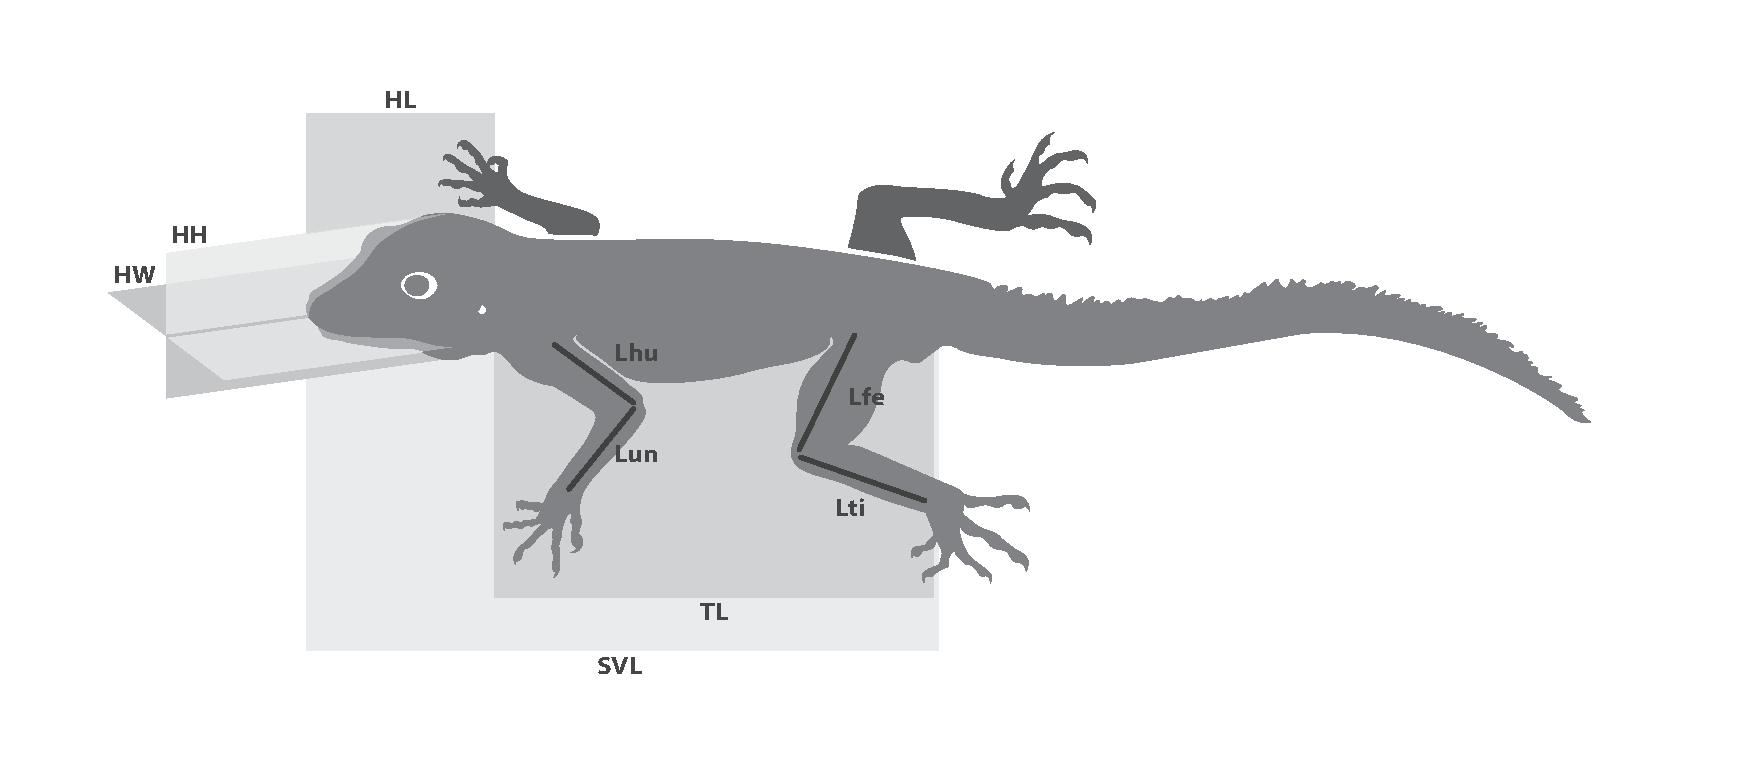
\includegraphics[width=1\linewidth]{Figs/Fig1} 

}

\caption{Linear Measurements used in this study. SVL = snout-vent length, TL = trunk length, HL = head length, HW = head width, HH = head height, Lhu = humerus length, Lun = ulna length, Lfe = femur length, Ltb = tibia length (for details see Tejero-Cicu{\'{e}}ndez et al. 2021a).}\label{fig:unnamed-chunk-4}
\end{figure}

\newpage

\begin{figure}

{\centering \includegraphics[width=1\linewidth]{Figs/figure_2_ggplot} 

}

\caption{Plot of regression scores and predicted lines representing the relationship between linear body measurements and size (SVL). Individuals are colored by habitat use: ground (beige), rock (dark purple), and tree (magenta). Isometric trend represented by the dashed line.}\label{fig:unnamed-chunk-5}
\end{figure}

\newpage

\begin{figure}

{\centering \includegraphics[width=1\linewidth]{Figs/figure_3_Pristurus_allometry_traitgram_legends} 

}

\caption{Traitgrams showing the evolution of body size (SVL) through time based on the phylogenetic tree of \textit{Pristurus}. Colors represent an evolutionary mapping of residuals from phylogenetic regressions describing the relationship of (A) head morphology versus body size, and (B) limb proportions versus body size (see text for descriptions). Species names are colored by habitat use: ground (beige), rock (dark purple), and tree (magenta).}\label{fig:unnamed-chunk-6}
\end{figure}

\newpage

\begin{figure}

{\centering \includegraphics[width=1\linewidth]{Figs/figure_4_static_allometry} 

}

\caption{Patterns of static allometry for each species for head traits (upper panel) and limb traits (lower panel). Species are separated by their habitat groups and colored by the magnitude of their regression slope (purple: steeper slopes, yellow: shallower slopes).}\label{fig:unnamed-chunk-7}
\end{figure}

\newpage

\begin{figure}

{\centering \includegraphics[width=1\linewidth]{Figs/figure_5_phylomorphospace_large_small} 

}

\caption{Phylomorphospace of \textit{Pristurus}, based on residuals from a phylogenetic regression of body measurements on size (SVL). Species means are colored by habitat use: ground (beige), rock (dark purple), and tree (magenta). Large and small rock-dwelling and ground-dwelling are highlighted with darker colors to highlight their differentiation and relative positions in morphospace.}\label{fig:unnamed-chunk-8}
\end{figure}

\newpage

\begin{figure}

{\centering \includegraphics[width=1\linewidth]{Figs/figure_6_Pristurus_allometry_rescaledSVL_horizontal} 

}

\caption{Representative specimens from large and small \textit{Pristurus} species, colored by habitat use: ground (beige) and rock (dark purple). Specimens are scaled to a common body size (SVL) to emphasize the relative differences in limb and head proportions. Original scale shown as the gray bar.}\label{fig:unnamed-chunk-9}
\end{figure}

\end{document}
